\documentclass[aspectratio=169,spanish]{beamer}
\usepackage{borelian}

\begin{document}
    \classtitle{3}{Estadística descriptiva}{6 de enero de 2026}

    \begin{frame}{Motivación}
        La estadística nos permite:

        \begin{itemize}
            \item \textbf{Describir} el comportamiento de fenómenos complejos utilizando conceptos sencillos (ejemplo: la media).
            %\item Capturar aspectos esenciales de su estructura y saber que tan incierto es el conocimiento generado.
            \item \textbf{Decidir}
            \item \textbf{Predecir}
        \end{itemize}

        En IA los datos son una parte fundamental para construir modelos precisos. La estadística es un área esencial, pues esta entrega herramientas y métodos para analizar y generar conocimiento sobre estos datos. 
    \end{frame}

    \begin{frame}[fragile]
    \frametitle{Ejemplo: Grasas saturadas y carbohidratos}

    En el estudio \textbf{PURE} realizado con $\sim$ 135000 personas se evaluó el riesgo de muerte según el consumo de carbohidratos y grasas saturadas.

    \begin{itemize}
        \item Los resultados muestran que un mayor consumo de carbohidratos esta ligado a una mayor tasa de muerte.

        \item Lo inverso ocurre para las grasas saturadas (resultado no esperado).
    \end{itemize}


    \end{frame}


    \begin{frame}[fragile]
    \frametitle{Ejemplo: Grasas saturadas y Carbohidratos}

    %El estudio \textbf{PURE} permitio:

    \begin{itemize}
        \item Resumimos un gran dataset en este gráfico esta generado solo con 10 valores. %es imposible ver los datos uno a uno 

        \item Hay mucha \textbf{incertidumbre} en los datos.
        
    \end{itemize}

    La Estadística proporciona herramientas nos ayuda a decidir que tan probable es que este experimento ocurra de forma aleatoria. 

    \end{frame}

    \begin{frame}[fragile]
    \frametitle{Principios de la Estadística}

    La Estadística se basa en los siguientes principios.

    \begin{itemize}
        \item \textbf{Aprender de los datos.} La estadística es un conjunto de herramientas para generar hipótesis de los datos.
        \item \textbf{Agregación.} En estadística resumimos un dataset completo calculando valores que describen la data.
        \item \textbf{Incertidumbre.} En el mundo estadístico siempre hay contraejemplos. Podemos cuantificar la incertidumbre.
        \item \textbf{Muestreo.} Queremos sacar conclusiones de una población sacando usando datos de una muestra.
        \item \textbf{Causalidad.} Algo causa otra cosa. 
    \end{itemize}
    \end{frame}

    \begin{frame}[fragile]
    \frametitle{Como aprendemos de los datos ? EDA }

    El \textbf{Análisis Exploratorio de Datos (EDA)} es un conjunto de técnicas que ayudan a entender un conjunto de datos.
    \vspace{5mm}
    \begin{itemize}
        \item El objetivo central es intentar encontrar patrones en los datos que nos permitan generar hipótesis. 
        \item Puede ser dividido en: descripción de los datos y visualización de los datos. 
    \end{itemize}

    \vspace{5mm}
    En esta clase hablaremos un poco sobre estadística descriptiva. En la siguiente clase ahondaremos en la visualizacion de datos.
    % Las \textbf{medidas de tendencia central} intentan resumir datos de un conjunto en un valor unico. 

    \end{frame}


    \begin{frame}[fragile]
    \frametitle{Medidas de tendencia central (Media)}

    Las \textbf{medidas de tendencia central} intentan resumir datos de un conjunto en un valor unico. 

    Dado un conjunto de datos $X =\{x_1,x_2,...,x_n\}$ la media se calcula como:

    \[ \text{Promedio}(X)=\bar{X} = \frac{1}{n} \sum^n_{i=1} x_i  \]

    El problema del promedio es que es muy sensitivo a \textbf{outliers} (valores atipicos).

    %Ejemplo:
    \begin{minted}{python}
    import numpy as np

    a = [1, 2, 3, 100]

    print( np.mean(a) ) # retornara  26.5
    print( mean(a) )    # retornara  26.5
    \end{minted}

    \end{frame}



    \begin{frame}[fragile]
    \frametitle{Valores atípicos}

    Como vimos la Media es afectada por outliers. Los outliers son valores atipicos en un conjunto de datos. Existen diferentes tipos de outliers:

    \vspace{5mm}

    %https://es.wikipedia.org/wiki/Media_%28matem%C3%A1ticas%29

    \end{frame}


    \begin{frame}[fragile]{Medidas de tendencia central: mediana}
        La mediana es el valor en la posición central de un conjunto de datos ordenado de menor a mayor o viceversa. Para un conjunto de datos \textbf{ordenado} $X =\{x_1,x_2,...,x_n\}$, se calcula como:

        \begin{equation*}
            \textsf{mediana}(X) = \begin{cases} 
                x_{(n+1)/2} & \text{si $n$ es impar} \\
                \frac{x_{n/2} + x_{n/2+1}}{2} & \text{si $n$ es par} 
            \end{cases}
        \end{equation*}

        En simple, es la observación que separa el conjunto de datos en una mitad de valores menores que él y otra mitad de valores mayores a él. 
        
        \begin{minted}{python}
            >>> import numpy as np

            >>> sample = [1, 2, 33, 100, 4]
            >>> np.median(sample)
        \end{minted}
    \end{frame}

    \begin{frame}[fragile]{Medidas de tendencia central: moda}
        La moda es el valor que aparece con mayor frecuencia en un conjunto de datos. Para un conjunto de datos $X =\{x_1, x_2, \dots, x_n\}$, se define como:

        \[
            \textsf{moda}(X) = \underset{x_i \in X}{\arg\max} \; f(x_i)
        \]

        donde $f(x_i)$ es la frecuencia de aparición del valor $x_i$ en el conjunto $X$.

        \begin{minted}{python}
            >>> from scipy import stats
            >>> sample = [1, 2, 2, 3, 4]
            >>> stats.mode(sample)
        \end{minted}
    \end{frame}

    \begin{frame}{Medidas de tendencia central: moda}
        La moda es especialmente útil para datos categóricos, donde la media y la mediana no son aplicables. Por ejemplo, en un conjunto de datos que representa colores favoritos, la moda sería el color que más personas prefieren.

        \begin{itemize}
            \item Un conjunto de datos puede tener más de una moda (bimodal, multimodal).
            \item La moda es menos sensible a valores atípicos en comparación con la media. ¿Se les ocurre por qué?
        \end{itemize}

        \begin{exampleblock}{Ejemplo}
            \begin{columns}
                \begin{column}{0.6\linewidth}
                    Consideremos el conjunto de datos simplificado que muestra las edades y alturas de tres personas.

                    ¿Cuál es la moda de las alturas? ¿Por qué? ¿Y la moda de las edades?                    
                \end{column}
                \hfill
                \begin{column}{0.3\linewidth}
                    \begin{table}[H]
                        \centering
                        \begin{tabular}{c|c|c}
                            $X$ & Edad & Altura (\textrm{m}) \\ \hline
                            $x_1$ & $17$ & $1.76$ \\
                            $x_2$ & $29$ & $1.76$ \\
                            $x_3$ & $10$ & $1.58$                
                        \end{tabular}
                    \end{table}
                \end{column}
            \end{columns}
        \end{exampleblock}
    \end{frame}

    \begin{frame}[fragile]
    \frametitle{Medidas de Tendencia Central (Percentiles)}
    La media puede ser generalizada con el concepto de percentil y quantil.

    \end{frame}

    \begin{frame}{La interpretación estadística \textbf{SÍ} importa}
        Consideremos un caso típico de análisis estadístico. Tomemos una muestra con $5$ chilenos, cada uno representado por una entrada en $X = \{x_1, x_2, x_3, x_4, x_5\}$, y sus respectivos sueldos:
        \begin{table}[H]
            \centering
            \begin{tabular}{c|c}
                $X$ & Sueldo (CLP) \\ \hline
                $x_1$ & $\$\, 300\,000$ \\
                $x_2$ & $\$\, 10\, 000\,000$ \\
                $x_3$ & $\$\, 75\,000$ \\
                $x_4$ & $\$\, 510\,000$ \\
                $x_5$ & $\$\, 7\,500\,000$
            \end{tabular}
            \caption{Sueldo mensual de una muestra de personas chilenas.}
            \label{tab:chilean-earnings}
        \end{table}
        \begin{itemize}
            \item ¿Cuál es el valor del promedio $\overline{X}$? ¿Y de $\textsf{mediana}(X)$?
            \item ¿Qué pasa si sólo nos enfocamos en informar sobre el promedio?
        \end{itemize}
    \end{frame}

    \begin{frame}{Medidas de dispersión}
        \begin{columns}
            \begin{column}{0.45\linewidth}
                \justifying
                \begin{block}{Definición}
                    \justifying
                    Las medidas de dispersión se vinculan con estadísticos que permiten describir la variabilidad de los datos en una muestra con respecto a una medida de tendencia central (usualmente la media).
                \end{block}
                La figura \ref{fig:scatter-variability} muestra la dispersión en un conjunto de puntos. \textbf{¿Cómo la resumimos en un número real?}
            \end{column}
            \begin{column}{0.5\linewidth}
                \begin{figure}[H]
                    \centering
                    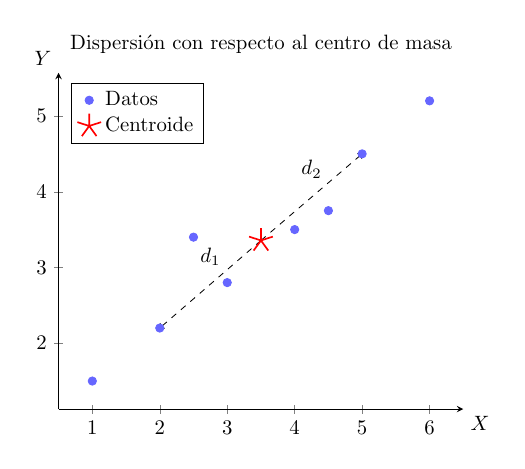
\begin{tikzpicture}[scale=0.75]
                        \def\dataset{1/1.5, 2/2.2, 3/2.8, 4/3.5, 5/4.5, 2.5/3.4, 4.5/3.75, 6/5.2}
                    
                        \def\sumx{0} 
                        \def\sumy{0} 
                        \def\countn{0}
                        \def\coords{}
                    
                        \foreach \x/\y in \dataset {
                            \pgfmathparse{\sumx+\x} \xdef\sumx{\pgfmathresult}
                            \pgfmathparse{\sumy+\y} \xdef\sumy{\pgfmathresult}
                            \pgfmathparse{\countn+1} \xdef\countn{\pgfmathresult}
                            
                            \xdef\coords{\coords (\x,\y)}
                        }
                    
                        \pgfmathsetmacro{\meanx}{\sumx/\countn}
                        \pgfmathsetmacro{\meany}{\sumy/\countn}
                    
                        \begin{axis}[
                            title={Dispersión con respecto al centro de masa},
                            axis lines=left,
                            xlabel={$X$},
                            ylabel={$Y$},
                            xlabel style={
                                at={(axis description cs:1,0)},
                                anchor=north west
                            },
                            ylabel style={
                                at={(axis description cs:0,1)}, 
                                anchor=south east,
                                rotate=-90
                            },
                            legend pos=north west,
                            legend cell align=left,
                            enlargelimits=0.1
                        ]
                            \addplot[only marks, mark=*, blue!60] coordinates {\coords};
                            \addlegendentry{Datos}
                            
                            \addplot[
                                only marks,
                                mark=star, 
                                mark size=6pt,
                                color=red,
                                thick
                            ] coordinates {(\meanx, \meany)};
                            \addlegendentry{Centroide}

                            \coordinate (centroid) at (\meanx, \meany);

                            \coordinate (point1) at (2, 2.2);
                            \coordinate (point2) at (5, 4.5);
                            
                            \draw[->,dashed] (centroid) -- node[above,yshift=2mm] {$d_1$} (point1);
                            \draw[->,dashed] (centroid) -- node[above,yshift=2mm] {$d_2$} (point2);
                        \end{axis}
                    \end{tikzpicture}
                    \caption{Dispersión de puntos en el espacio $\mathbb{R}^2$.}
                    \label{fig:scatter-variability}
                \end{figure}
            \end{column}
        \end{columns}
    \end{frame}

    \begin{frame}[fragile]{Medidas de dispersión: varianza}
        La varianza mide qué tan dispersos están los datos con respecto a la media aritmética. Para un conjunto $X = \{x_1, x_2, \dots, x_n\}$, se puede calcular como:

        \[ 
            \mathbb{V}\textsf{ar}(X) = \frac{1}{N-1} \sum^n_{i=1} \left(x_i - \bar{X}\right)^2 
        \]

        \begin{minted}[escapeinside=||]{python}
            >>> import numpy as np

            >>> |$\ell$| = [8, 3, 5, 10]
            >>> np.var(|$\ell$|)
        \end{minted}

        \textbf{Pregunta}: ¿Cuál es la varianza de la muestra $X = \{1, 1, \dots, 1\}$ (sólo unos)?
    \end{frame}


    \begin{frame}[fragile]
    \frametitle{Medidas de variabilidad: varianza}
    Para cuantificar cuanto varia una variable con respecto a otra utilizamos metricas multivariadas. 

    La \textbf{covarianza} \emph{cov(x,y)} mide el grado de cambio lineal en conjunto de dos variables $x,y$.

    \[ \textrm{cov}(X,Y) = \frac{1}{n-1} \sum^n_{i=1} (x_i - \bar{X}) (y_i - \bar{Y}) \]

    \begin{lstlisting}[language=Python]
    import numpy as np

    X = [42,9,21,31]
    Y = [3,2,1,11]
    print(np.cov(X,Y)) # retornara la covarianza entre a y b

    \end{lstlisting}


    \end{frame}


    \begin{frame}[fragile]
    \frametitle{Medidas de variabilidad  (Co-Varianza y Correlacion)}
    \vspace{5mm}
    \begin{itemize}
        \item Si dos variables $X,Y$ son independientes, entonces su covarianza sera 0.
        
        \item Si dos variables $X,Y$ son dependientes, entonces diremos que existe una \textbf{correlacion} entre estas.
    
    \end{itemize}

    Una metrica bastante importante es la correlacion lineal $r(x,y)$, que estima la relacion entre dos variables (covarianza) independiente de su magnitud.

    \[
    r(x,y) = \frac{cov(x,y)}{sd(x)sd(y)}
    \]

    \end{frame}



    \begin{frame}[fragile]
    \frametitle{Resultado fundamental: correlación $\not\Rightarrow$ causalidad}

    % El bloque de pregunta siempre es visible
    \begin{block}{Pregunta}
        Si $x + 2 = 5$, ¿cuánto vale $x$?
    \end{block}

    \pause % Espera un click

    % El bloque de respuesta aparece después
    \begin{exampleblock}{Solución}
        Restamos 2 a ambos lados:
        $$ x = 5 - 2 = 3 $$
    \end{exampleblock}

    \textbf{Pregunta:} Si dos variables $X$ e $Y$ están correlacionadas, ¿significa esto que $X$ \textbf{causa} a $Y$ o viceversa?

    No necesariamente, pueden existir variables ocultas.
    \end{frame}



    \begin{frame}[fragile]
    \frametitle{Variables aleatorias}

    \begin{block}{Definición: \textit{Variable aleatoria}}
        Una variable aleatoria (abreviada v. a.) $X$ representa 
    \end{block}

    \end{frame}

    \begin{frame}{Referencias}
        \begin{itemize}
            \item Statistical Thinking for the 21st Century. 2019. Russell A. Poldrack. \url{https://statsthinking21.github.io/statsthinking21-core-site/}
        \end{itemize}
    \end{frame}
\end{document}